Many notes together form patterns, many patterns form a beatmap (short: map).
Each beatmap corresponds to a piece of music.

\begin{figure}[H]
    \centering
    \begin{verbatim}
     ^ |         | End of Song
     | | O O   O |
     | |         |
     | |   O O   | ^
 Map | | O       | | Pattern
     | |   O O | | v 
     | |       | | 
     | | O O O O | 
     v | ======= | Start of Song
         Receptor
    \end{verbatim}
    \caption{Difference between Map and Pattern}
    \label{fig:pattern_map}
\end{figure}

Think of an art piece: a pattern within the art is a subset of the art piece.
However, the definition is loose, the pattern may be the whole art piece.


\section{Judgements}\label{sec:judgements}

Judgements determine the quality of your rhythm.
If you pressed the key on time, it'll give a better judgement.
Judgements will dictate the overall score and rhythmic accuracy of the play.

\begin{figure}[H]
    \centering
    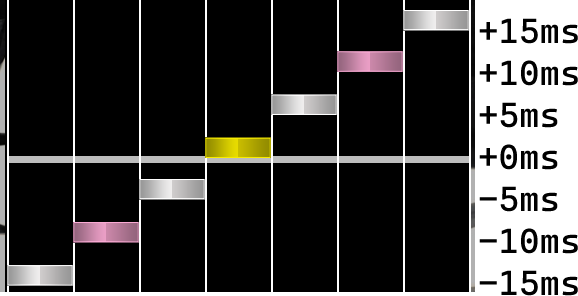
\includegraphics[scale=0.25]{imgs/judgement}
    \caption{Judgements depending on how early or late the player hits.}
    \label{fig:judgement}
\end{figure}

For example, judgements in osu!
are as follows for overall difficulty\footnote{overall difficulty affects strictness of these judgement windows} of 8.
\begin{table}[H]
    \centering
    \begin{tabular}{c|c}
        Window       & Judgement                                             \\  \hline
        $\pm16.5ms$  & Best\footnote{These are not exact terms used by osu!} \\
        $\pm40.5ms$  & Good                                                  \\
        $\pm73.5ms$  & Okay                                                  \\
        $\pm103.5ms$ & Not Good                                              \\
        $\pm127.5ms$ & Bad                                                   \\
        otherwise    & Miss                                                  \\
    \end{tabular}
    \caption{Judgement Windows for osu!}
    \label{tab:judgement_osu}
\end{table}

